\newpage
\chapter{Modules}\textit{Theis.}\\
This chapter is about the information web page for the energy hub. The purpose of this web page and the thought about designing it, and how it will work is described here.
\section{Design Ideas}
The purpose of the hub web page is to see what type of module that is connected to which ports, and to see the production versus the consumption. It is also possible to see some status of the energy hub. The design shall be simple, and it have to be a web page without to many things to distract the users. To fulfil this, there have been made 3 regions in the page window, one with the graph, one for data and status, and a third one for the modules.\\
To keep dynamic on the homepage, the design from the index page, has been kept through the web site. The background color is the same, and the dock in the bottom is kept on all sub pages. A big headline is made with an icon, to show what page the user is looking at.
\section{The Design}

\begin{figure}[h!]
	\center
		\setlength\fboxsep{0pt}
		\setlength\fboxrule{1pt}
		\fbox{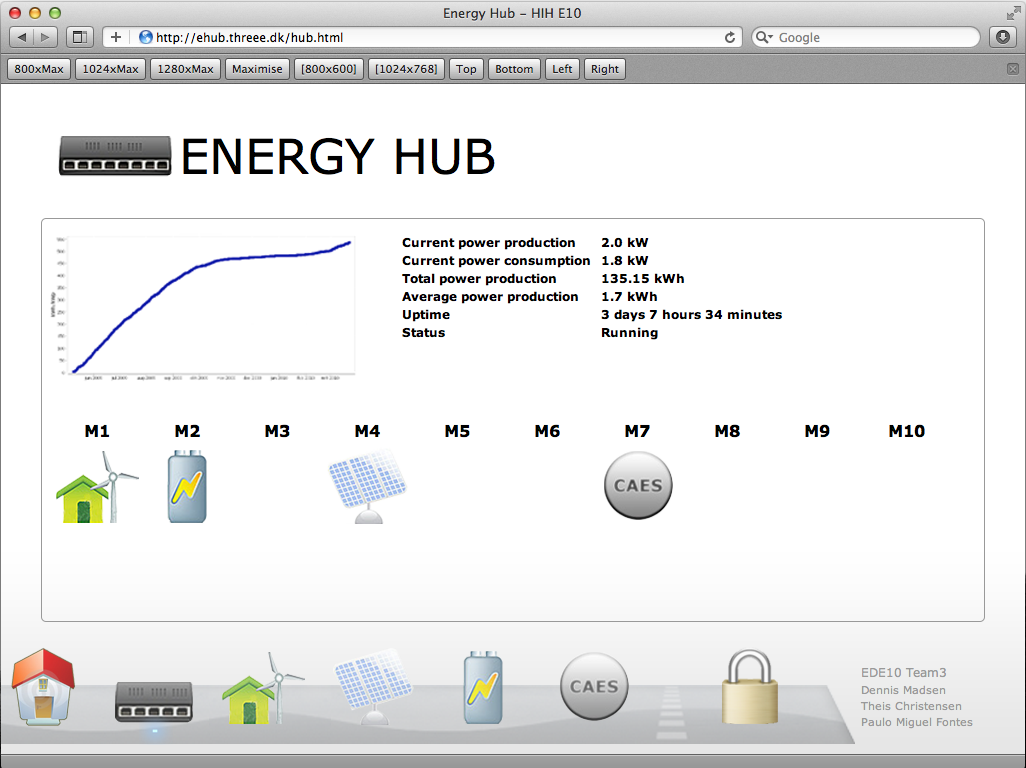
\includegraphics[width=0.55\textwidth]{images/screen_hub_page.png}}
   	\caption{Picture of the hub page.}
   	\label{fig:hub_page_design}
\end{figure}
This is how the design turns out. It fulfills the purpose and the requirements for the design (simple and easy to navigate).
\section{Code layout}
Here is a description of the code settings and layout that is used for the web page.
\subsection{Doctype}
In this project the document type XHTML 1.0 Strict is used. The DOCTYPE declaration tells the browser how to interpret the code in which the site is written. It should be written at the first line in every valid html file, as seen in the code below. This type has every feature of the HTML. The markup must be written as well formed XML. Strict, in contrary to Transitional, document types does not include deprecated tags (e.g. \textless font\textgreater , \textless target\textgreater), so all the styling is made in CSS style sheet.
\begin{lstlisting}
<!DOCTYPE html PUBLIC "-//W3C//DTD XHTML 1.0 Strict//EN" "http://www.w3.org/TR/xhtml1/DTD/xhtml1-strict.dtd">
<html>
	<head></head>
	<body>
	</body>
</html>
\end{lstlisting}

\subsection{Meta tag}
The meta tags tell something about the data on the page. In the first line the content type is set to "text/html" this means that the browser will show the page as normal, the charset is also set in that line to "UTF-8". The second line is for the mobile version of the web page (will be explained in the next chapter).
\begin{lstlisting}
<meta http-equiv="Content-Type" content="text/html; charset=UTF-8" />
<meta name="viewport" content="width=device-width, initital-scale=1, user-scalable=no" />
\end{lstlisting}

\section{Code explanation}
Here the code will be described and shown in pieces
\subsection{Division}
The "div" tag is used to make sections in a html document, it is then easy to set up some style settings in the css file. Below is some code with two div tags. The divisions have the same class but two different ids.
\begin{lstlisting}
<div class="modules" id="M1">		
	M1<br /><a href="../wind/"> <img src="/pic/dock_wind.png" alt="WIND_module"/> 	</a>
</div>
<div class="modules" id="M2">
	M2<br /><a href="../battery/"> <img src="/pic/dock_bat.png"  alt="battery_module"/>	</a>
</div>
\end{lstlisting}
The class and ids is very handy in css. In the code below there is some settings for the class named "modules", these settings is for the whole class, this means that the two divisions above have the same style settings. From line 10 and down, in the code below some settings for the specific id. The css code here sets up some common style settings for the class and then the divisions is moved away from the left side as the id gets higher.
\begin{lstlisting}[language=CSS]
/*MODULES*/
.modules {/*Classe settings*/
	text-align: center;
	font-weight: bold;
	position:inherit;
	height: 120px;
	width: 90px;
	top: 200px;
}
/*Setting for single id*/
#M1	{left: 10px;}
#M2	{left: 100px;}
\end{lstlisting}

\subsection{Headings}
Headlines in html can be made with headings tags (\textless h1\textgreater  to\textless h6\textgreater). The specific look of the headings is then defined in the css file. The h1 tag is used in the html code below.
\begin{lstlisting}
<div id="header">
	<img src="/pic/hub.png" alt="HUB_module"/>
	<h1>ENERGY HUB</h1>
</div>
\end{lstlisting}
The code below is the css code to design the h1 tag from the html code above. In the css code the font size of h1 in the header division is set to 48px, the top padding is also set, which is the space from the element above the heading and to the text in the heading.
\begin{lstlisting}[language=CSS]
#header h1{ font-size: 48px; padding-top: 35px;}
\end{lstlisting}

\subsection{Table}
To show the data for the hub a table is used, this is done in html as shown in the code below. The table starts in line 2. The "tr" tag makes a row, and the "td" tag define the cells in the row.
\begin{lstlisting}
<table>
	<tr>
		<td>Current power production</td><td>2.0 kW</td>
	</tr>
	<tr>
		<td>Current power consumption</td><td>1.8 kW</td>
	</tr>
	<tr>
		<td>Total power production</td><td>135.15 kWh</td>
	</tr>
	<tr>
		<td>Average power production</td><td>1.7 kWh</td>
	</tr>
	<tr>
		<td>Uptime</td><td>3 days 7 hours 34 minutes</td>
	</tr>
	<tr>
		<td>Status</td><td>Running</td>
	</tr>
</table>
\end{lstlisting}
The css for the table is seen below, here the space to the left side of each cell is set, the font is set to bold, and the font size is set to 12px.
\begin{lstlisting}[language=CSS]
#status td {
	padding-left: 10px;
	font-weight: bold;
	font-size: 12px;
}
\end{lstlisting}

\subsection{General tags}
A css file that determine the design of html file needs to be include in the html, this is done in the line 2 to 4. If a html page has more than one css file, then it will use every file, but if one thing is defined in two files the file that are listed last will be used. Images is included in html as in line 6, the "img" tag says that this is an image, the "src" defines the source, where to find the file, the "alt" is alternative text if the file cannot be found. In line 7 a link is defined, the "a" makes a link the "href" is the reference where the link points to, the text "link" between the "a" tag is what is shown on the page, this could also be a image, then the image will work as a link.
\begin{lstlisting}
<!--include css files-->
<link rel="stylesheet" type="text/css" href="/reset.css" />
<link rel="stylesheet" type="text/css" href="../styles.css" />
<link rel="stylesheet" type="text/css" href="style_hub.css" />
<!--include css files-->
<img src="/pic/background.png" alt="background"/>
<a href="/">link</a>
\end{lstlisting}
In the css code it is possible to make design of the html code, in the css code below there is some commands that can be set. In the first line the position of the element is set, this can be set to absolute there the position is define from the top left corner of the browser, below it is set to inherit, this means that the position is define from the division, in the code below the top and left command determines the space from the top left corner in the division, this could also be bottom and right. The height and width sets the size of the division. The border command makes a boarder around the division with a width of 1px and the color \# 999. The border-bottom-left-radius is a css 3 tag. this make a round corner with a radius of 5px.
\begin{lstlisting}[language=CSS]
position:inherit;
height: 200px;
width: 400px;
left: 350px;
top: 15px;
border: 1px solid #999;
border-bottom-left-radius: 5px;
\end{lstlisting}